\chapter{Introduction}
The purpose of this project is to design a dashboard with financial and economical KPIs, in order to provide trends and values to verify and monitor the company's performances. We have 

We expanded the work, adding a new objective, as shown in the figure \ref{fig:concmap} below, representing the general outline of our project.


\begin{figure}[h]
    \centering
    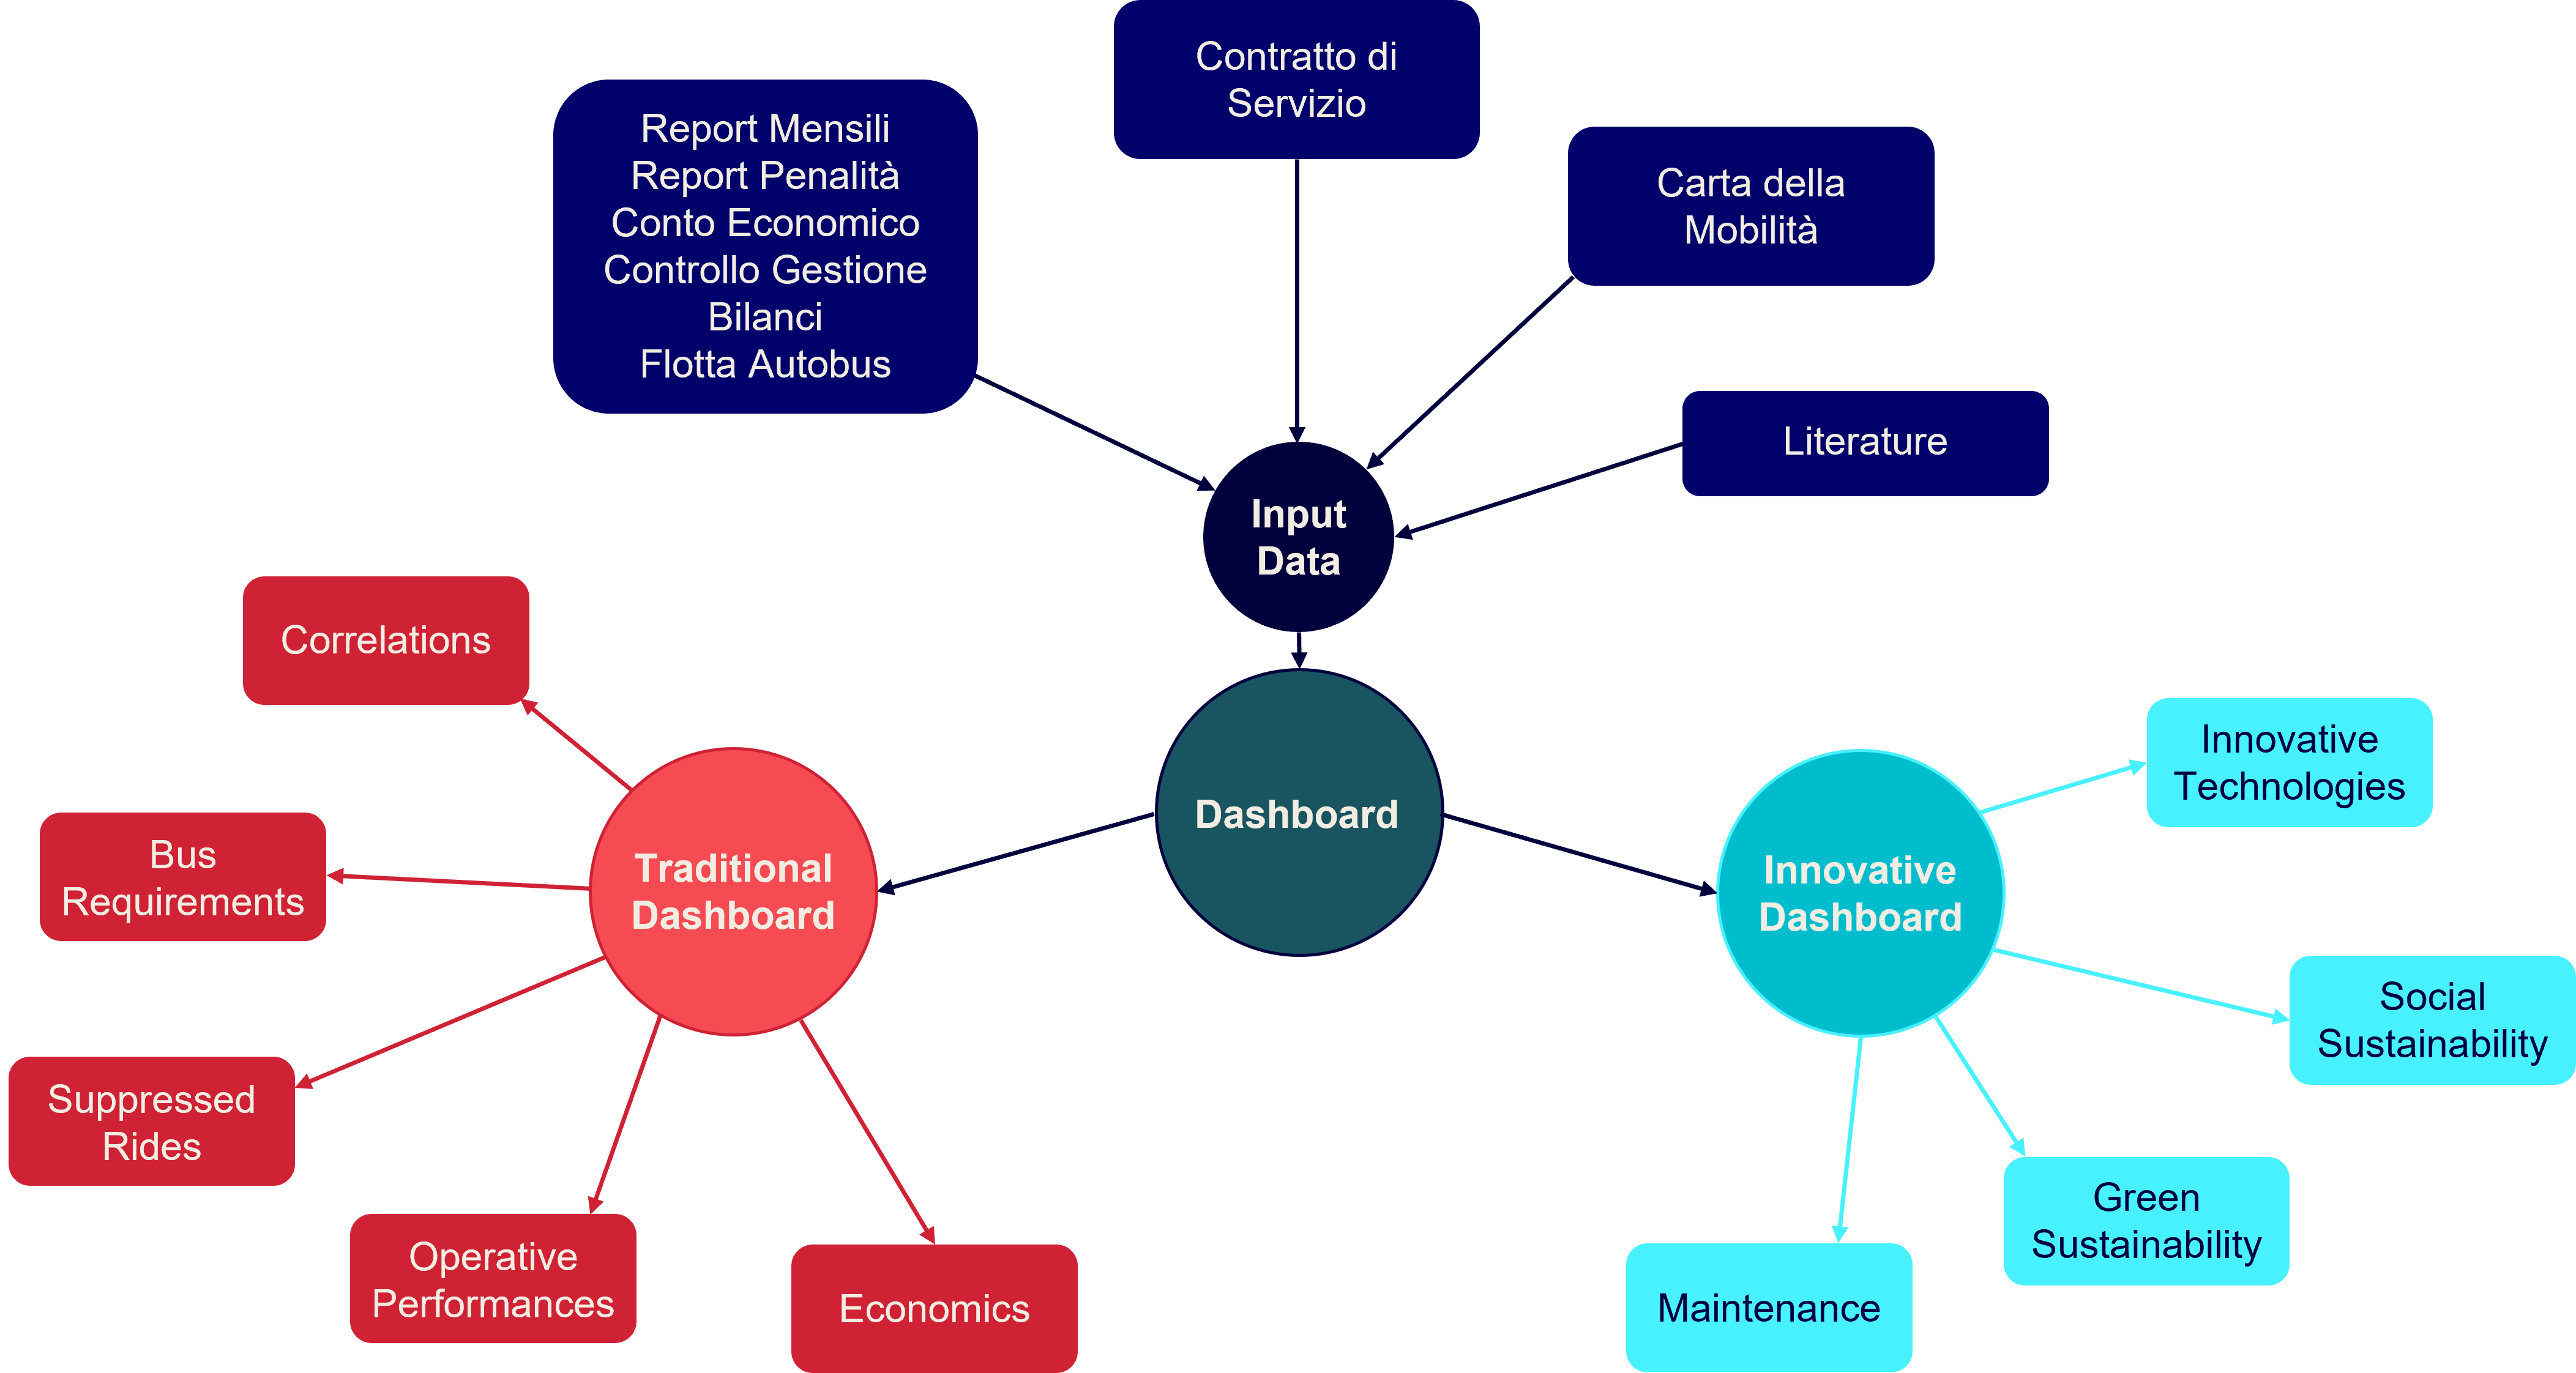
\includegraphics[width=1\textwidth]{Images/intro_scheme.png}
    \caption{Conceptual Map of the work}
    \label{fig:concmap}
\end{figure}

First of all, a presentation of the study case has been made with an analysis of the service
contract and a short history recap of the public service in the Subnetwork SUD of the
Province of Bergamo (that starts in 2004). From this, we have been found some KPIs useful
to monitor and check the compliance with the requirements of the service contract (for
example: bus fleet requirements, suppressed rides, ...).

Using the datasets provided by Arriva we first have done a data cleaning, in order to create a dashbpard that could work on three main levels: consortium's companies, lines and time (month or year). Along with the dashboard a work of investigation and comment of the result have been presented with the aim of discuss and highlight the potential of the work.

Taking in consideration also the current changes in the world and in particular in the mobility sector (COVID-19 before and now the energy crisis due to Ukraine war) and  the objectives of ONU \cite{sdgs}, the second part talk about how to implement new aspects of this sector in a new and innovative dashboard; we will assess analyses on new technologies of public transport, different perspectives on sustainability such as green and social, concluding with a focus on maintenance procedures of new buses.

%FINITO
\date{\today}
















